\documentclass[11pt]{beamer}
\usetheme{simple}
\setbeamertemplate{footline}{} 
\usepackage{tikz}

\usepackage{pgfplots}
\usepackage{amsmath, amssymb, amsthm}   
\pgfplotsset{
        % declare the function you want to plot so you can reuse it easily later
        /pgf/declare function={
            T1(\u)=ln(0.5*(-2*\u+sqrt(4+4*\u^2)));
            T0(\u)=ln(0.5*(2*\u+sqrt(44+4*\u^2)));     
            U0(\u)=\u-1;
            T12(\u)=ln(-1-2*\u);
        },
        % define style to use for the plot to draw only ticks at `\myxlist'
        % (the plot should be invisible)
        my ticks/.style={
            samples at={\myxlist},
            mark=none,
            draw=none,
%            only marks,     % <-- uncomment me to show the data points
        },
every non boxed y axis/.append style={y axis line style=-}
    }
%\pgfplotsset{ every non boxed y axis/.append style={y axis line style=-}}
\setbeamertemplate{navigation symbols}{}
\begin{document}
\begin{frame}

\tikzset{every picture/.style={line width=0.75pt}} %set default line width to 0.75pt        

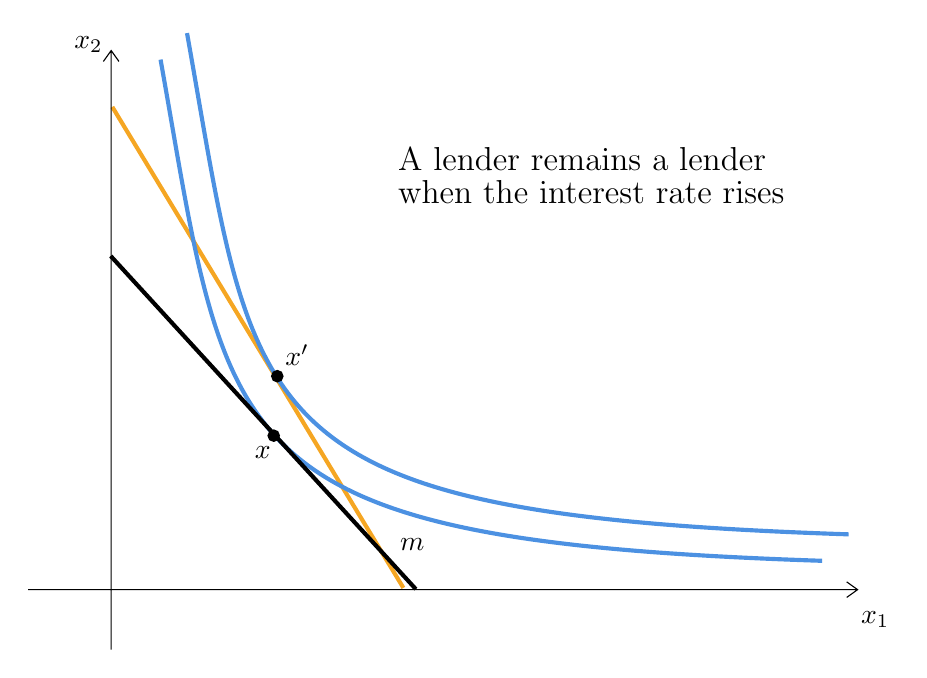
\begin{tikzpicture}[x=0.75pt,y=0.75pt,yscale=-.75,xscale=.75]
%uncomment if require: \path (0,443); %set diagram left start at 0, and has height of 443

%Straight Lines [id:da17537097093516762] 
\draw [color={rgb, 255:red, 245; green, 166; blue, 35 }  ,draw opacity=1 ][line width=1.5]    (107.3,72.8) -- (294.3,381.8) ;


%Shape: Axis 2D [id:dp11877989343343409] 
\draw  (53.3,382.93) -- (586.09,382.93)(106.58,36.6) -- (106.58,421.41) (579.09,377.93) -- (586.09,382.93) -- (579.09,387.93) (101.58,43.6) -- (106.58,36.6) -- (111.58,43.6)  ;
%Curve Lines [id:da6451900492142217] 
\draw [color={rgb, 255:red, 74; green, 144; blue, 226 }  ,draw opacity=0.99 ][line width=1.5]    (138.3,42.4) .. controls (183.3,294.4) and (171.3,351.4) .. (563.3,364.4) ;


%Straight Lines [id:da3745755779223563] 
\draw [line width=1.5]    (106.3,168.6) -- (302.3,382.6) ;


%Straight Lines [id:da6976937457559602] 
\draw    (211,284) ;

\draw [shift={(211,284)}, rotate = 0] [color={rgb, 255:red, 0; green, 0; blue, 0 }  ][fill={rgb, 255:red, 0; green, 0; blue, 0 }  ][line width=0.75]      (0, 0) circle [x radius= 3.35, y radius= 3.35]   ;
%Curve Lines [id:da6659329280855124] 
\draw [color={rgb, 255:red, 74; green, 144; blue, 226 }  ,draw opacity=0.99 ][line width=1.5]    (155.3,25.4) .. controls (200.3,277.4) and (188.3,334.4) .. (580.3,347.4) ;


%Straight Lines [id:da2195902947773971] 
\draw    (213.3,245.8) ;

\draw [shift={(213.3,245.8)}, rotate = 0] [color={rgb, 255:red, 0; green, 0; blue, 0 }  ][fill={rgb, 255:red, 0; green, 0; blue, 0 }  ][line width=0.75]      (0, 0) circle [x radius= 3.35, y radius= 3.35]   ;

% Text Node
\draw (597.35,402.33) node   {$x_{1}$};
% Text Node
\draw (92,33) node   {$x_{2}$};
% Text Node
\draw (415,117) node  [align=left] {{\large A lender remains a lender}\\{\large when the interest rate rises}};
% Text Node
\draw (300,354) node   {$m$};
% Text Node
\draw (204,295) node   {$x$};
% Text Node
\draw (226,232) node   {$x'$};


\end{tikzpicture}
\end{frame}
\end{document}
